\chapter{Experiments}\label{cha:experiments}

\section{Simulator}\label{sec:simulator}

We created a simulator to generate distorted points as described in
\cref{sub:complete_projection_and_backprojection}. We used it to test the
solver and test the correctness of projection and back-projection points.
However, since the simulator used the same camera model as the solver, the
initial camera calibration was perfect.

\section{Metrics}\label{sec:metrics}

As noted by \cite{duisterhofTartanCalibIterativeWideAngle2022}, the evaluation
of the camera calibration is not straightforward. No ground truth exists for
feature detection or camera calibration.

Typically, the reprojection error is used as a metric for the camera
calibration, but it depends on multiple factors: type of the calibration
pattern, the camera model, and the types of the lens.

Also, by using more features, we can get better calibration, as we have more
constraints, but the reprojection error might be higher.

As currently the algorithm only supports processing a single checkerboard, we
cannot compare to \cite{duisterhofTartanCalibIterativeWideAngle2022}, which uses
AprilTags, nor to the \cite{lochmanBabelCalibUniversalApproach2021}, who
provides the detected corners for all of the boards.
\todo{Should I maybe tell less about it?}

Because of that, we instead artificially removed some of the points from the
detections, to ensure that we can recover them. We also created
artificially occluded points by overlaying a separate image, as it poses
problems for the feature detector.

Lastly, we evaluated the newly detected points on real-world datasets.

\section{Dataset}\label{sec:dataset}

For the project, we need highly distorted photos of calibration boards. It takes
a lot of work to generate such a dataset, as cameras which produce such images are
usually expensive. Therefore, it would be preferable to use an existing dataset.

For this project, we required a highly distorted dataset of chessboard images.
We collected several datasets, but the feature detector we used supports
detecting only the boards with the constant tile size, therefore we cannot use
AprilGrid nor CharuCO boards. The feature detector is the only limiting factor.

\textcite{lochmanBabelCalibUniversalApproach2021} collected a wide number of
datasets, typically used in the field for the benchmarking of the camera
calibration. They're provided in a Deltille \cite{DeltilleDetector2023} format,
and are well documented:

\textbf{Kalibr} \citep{mayeSelfsupervisedCalibrationRobotic2013} contains several established datasets that are commonly used for testing
the accuracy of camera calibration frameworks: Double Sphere
\cite{usenkoDoubleSphereCamera2018}, EuRoC \cite{burriEuRoCMicroAerial2016}, TUM
VI \cite{schubertTUMVIBenchmark2018}, and ENTANIYA 1
\cite{Calibration250degFisheye}.
The Kalibr calibration framework was used in the
original publications cited above, hence the name of the dataset.
As a calibration pattern, AprilGrid with 6x6 tags of 88 mm size was used.
In total, the datasets contain approximately 800 images.

\textbf{OCamCalib} \citep{scaramuzzaFlexibleTechniqueAccurate2006} is a dataset
of approximately 300 images.
As a calibration pattern, the checkerboard pattern of different sizes was used.

\textbf{UZH} \citep{AreWeReady} is a dataset of approximately 800 images
collected using the following cameras:
As a calibration pattern, AprilGrid with 4x5 tags of 75 mm size was used.
The dataset contains approximately 800 images.

\textbf{OV} \citep{lochmanBabelCalibUniversalApproach2021} is a dataset of
approximately 1400 images. It was collected using eight stereo cameras.
As a calibration pattern, the checkerboard pattern with 9x6 tags of 22 mm size
was used.

\textcite{duisterhofTartanCalibIterativeWideAngle2022} also provide their
dataset from the TartanCalib project. Currently, the dataset contains only
AprilGrid patterns, as the toolchain doesn't support a chessboard.

\begin{figure}[h]
	\centering
	\begin{subfigure}[b]{0.3\linewidth}
		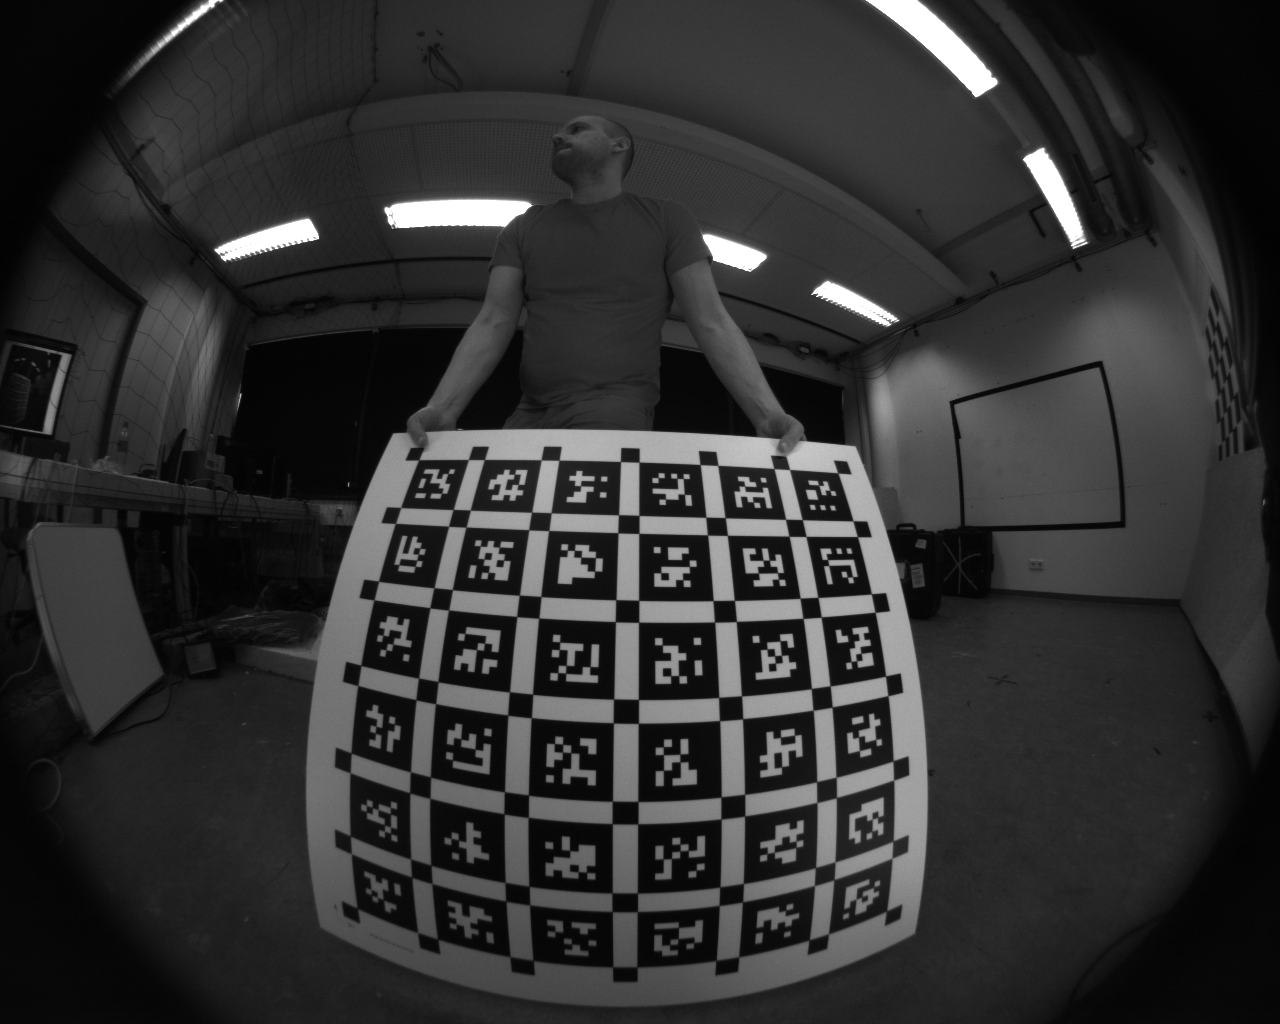
\includegraphics[width=\linewidth]{Kalibr.png}
		\caption{Kalibr}
	\end{subfigure}
	\hfill
	\begin{subfigure}[b]{0.3\linewidth}
		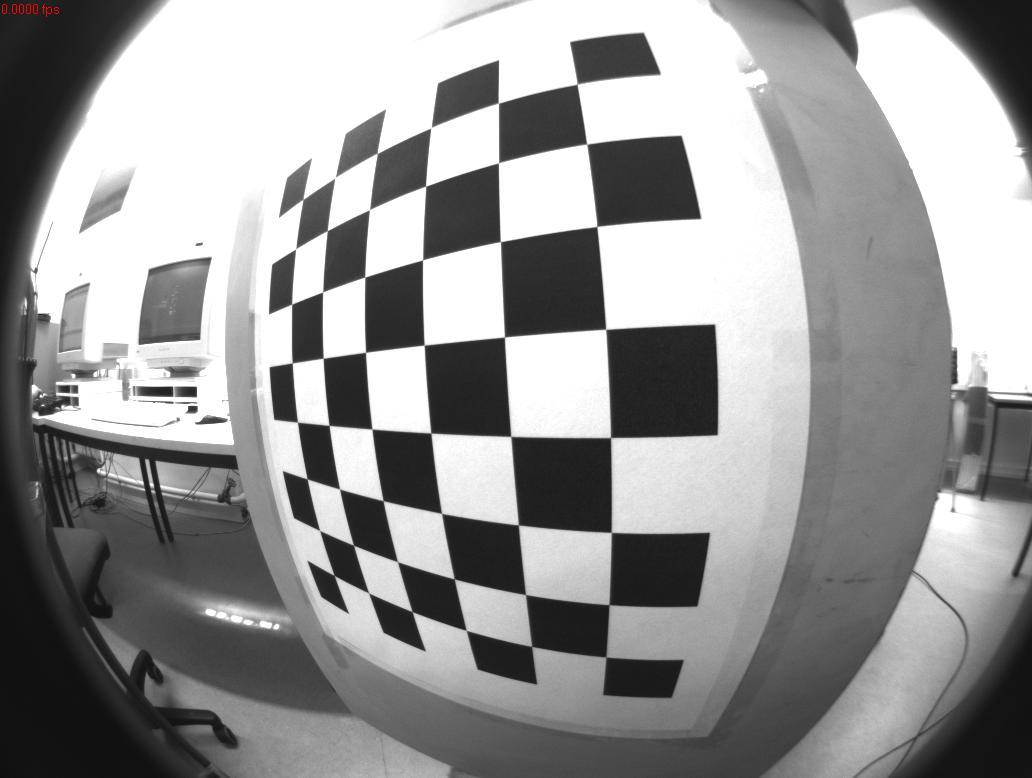
\includegraphics[width=\linewidth]{OCamCalib.png}
		\caption{\textbf{OCamCalib}}
	\end{subfigure}
	\hfill
	\begin{subfigure}[b]{0.3\linewidth}
		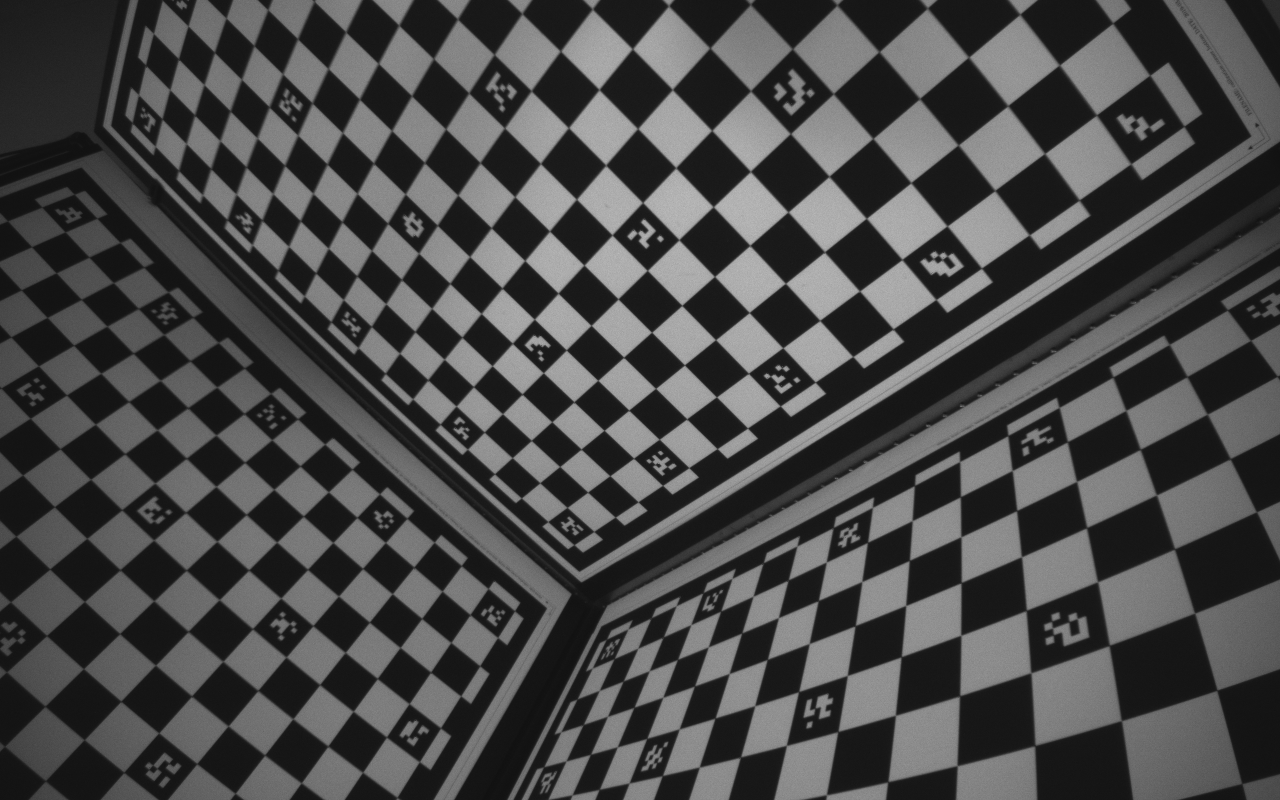
\includegraphics[width=\linewidth]{OV.png}
		\caption{\textbf{OV}}
	\end{subfigure}
	\begin{subfigure}[b]{0.3\linewidth}
		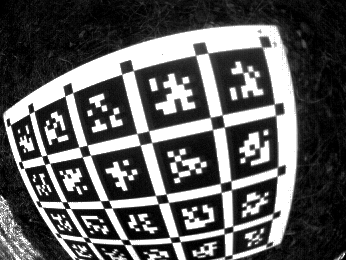
\includegraphics[width=\linewidth]{UZH.png}
		\caption{UZH}
	\end{subfigure}
	\begin{subfigure}[b]{0.3\linewidth}
		\includegraphics[width=\linewidth]{tartancalib.png}
		\caption{TartanCalib}
	\end{subfigure}
	\caption{Images from the datasets}
\end{figure}

\section{Camera calibration}\label{sec:camera_calibration}

\begin{minipage}{0.5\linewidth}
	To get accurate predictions for the possibly missing points, we need
	very accurate camera calibration. We used the reprojection error as a metric
	for the calibration quality.
	To calculate the reprojection error, we have to perform the
	rootfinding \cref{subsub:back_projection_using_the_division_model}. We assume
	that all of the points lay within the image, or they get out of the borders
	a little bit (we use the constant \(1.1\) of the maximum radius). If the
	camera calibration is poor, the root-finding might fail. On the initial
	calibration the number of the failed root-findings was much higher.
\end{minipage}
\hfill
\begin{minipage}{0.4\linewidth}
	\resizebox{\linewidth}{!}{
		\begin{tikzpicture}
			\pie[rotate=90, explode=0.1, sum=auto, color={green!60, blue!60, red!60}, text=legend]{
				115/Correctly detected,
				80/Reprojection error > 10,
				254/Not correctly detected
			}
		\end{tikzpicture}
	}
	\captionsetup{width=.9\linewidth}
	\captionof{figure}{Initial calibration}
	\resizebox{\linewidth}{!}{
		\begin{tikzpicture}
			\pie[rotate=90, explode=0.1, sum=auto, color={green!60, blue!60, red!60}, text=legend]{
				658/Correctly detected,
				19/Reprojection error > 10,
				115/Not correctly detected
			}
		\end{tikzpicture}
	}
	\captionsetup{width=.9\linewidth}
	\captionof{figure}{Final calibration}
\end{minipage}

% \begin{figure}[h]
% 	\begin{tikzpicture}
% 		\begin{axis}[
% 				ybar interval,
% 				ymin=0,
% 				ylabel={Frequency},
% 				xlabel={Value},
% 				height=0.3\linewidth,
% 				width=\linewidth,
% 				ticklabel style = {font=\tiny},
% 				% title={Initial calibration}
% 			]
% 			\addplot+ [hist={data min=0,data max=10,bins=20}] table [y index=0]
% 				% \addplot+ [hist={bins=30}] table [y index=0]
% 				{data/reprojection_error_init.txt};
% 		\end{axis}
% 	\end{tikzpicture}
% 	\caption{Initial calibration's reprojection error histogram}
% \end{figure}
% \begin{figure}[h]
% 	\begin{tikzpicture}
% 		\begin{axis}[
% 				ybar interval,
% 				ymin=0,
% 				ylabel={Frequency},
% 				xlabel={Value},
% 				height=0.3\linewidth,
% 				width=\linewidth,
% 				ticklabel style = {font=\tiny},
% 				% title={Reprojection error}
% 			]
% 			\addplot+ [hist={data min=0,data max=10,bins=20}] table [y index=0]
% 				% \addplot+ [hist={bins=30}] table [y index=0]
% 				{data/reprojection_error_final.txt};
% 		\end{axis}
% 	\end{tikzpicture}
% 	\caption{Final calibration's reprojection error histogram}
% \end{figure}
\todo{Add data and enable}

\section{Additional features detection}\label{sec:additional_features_detection}

As discussed in \cref{sec:additional_features_detection}, we filled the gaps in
the originally detected board points, and then padded it for 1 additional
element.

\begin{figure}[h]
	\centering
	\begin{minipage}{0.55\linewidth}
		\begin{subfigure}[b]{\linewidth}
			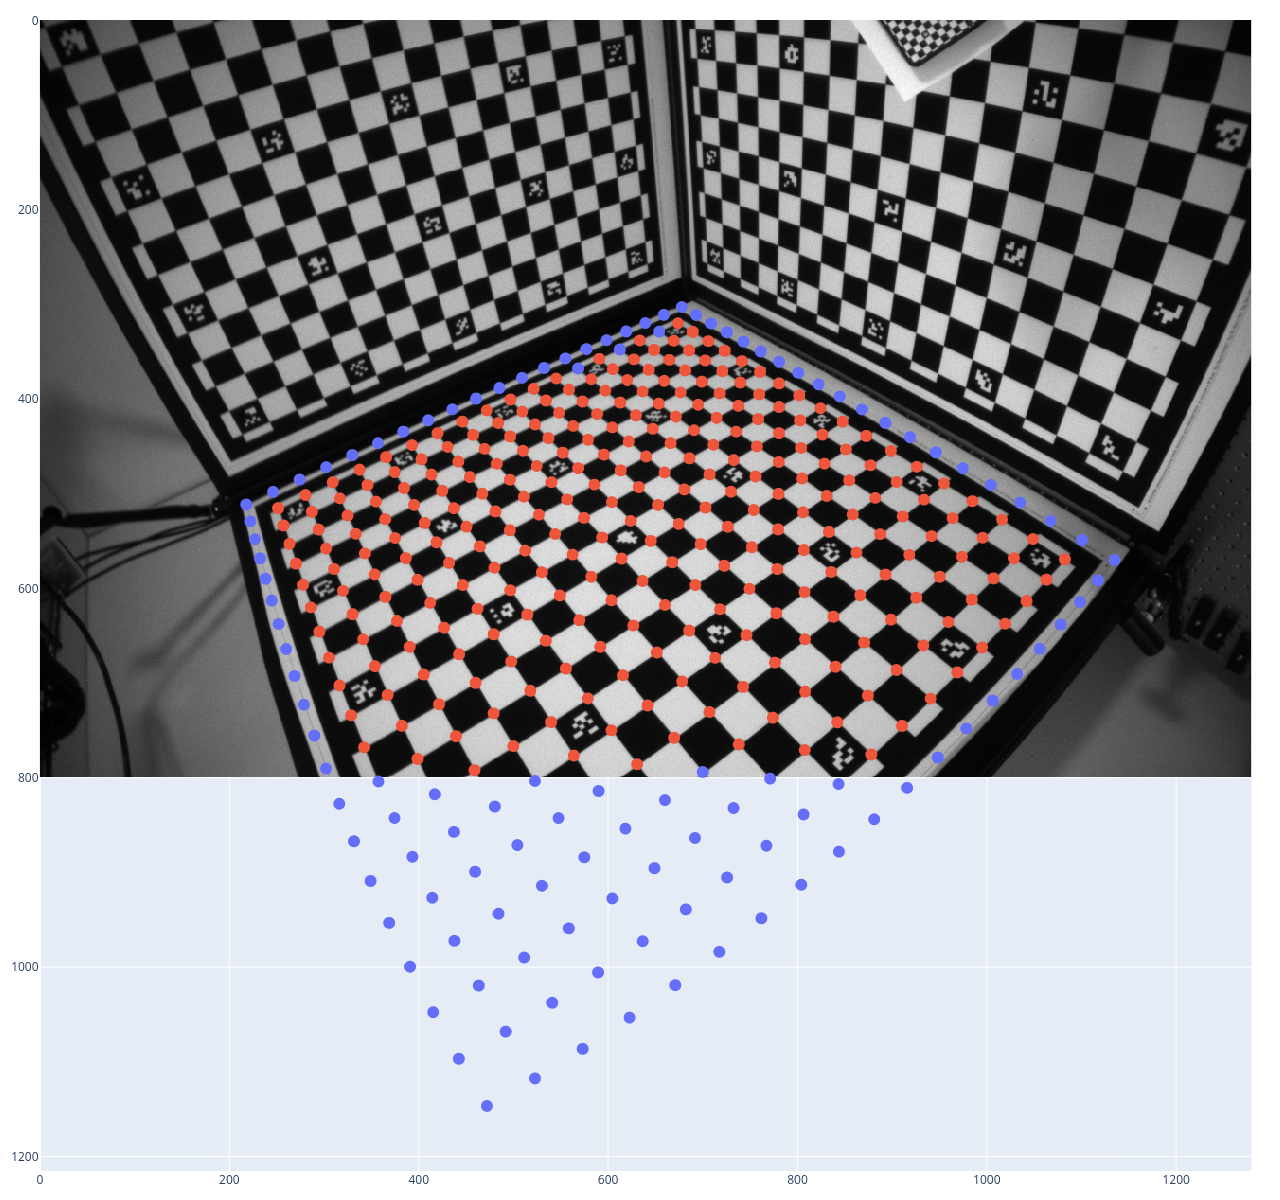
\includegraphics[width=\linewidth]{extended_board_img.png}
			\label{fig:extended_board_img}
			\caption{Extended board, new points are marked as blue}
		\end{subfigure}
	\end{minipage}
	\begin{minipage}{0.35\linewidth}
		\resizebox{\linewidth}{!}{
			\begin{tikzpicture}
				\begin{axis}[
						xlabel={$x$},
						ylabel={$y$},
						grid=major,
						title={Original board},
					]
					\addplot[
						only marks,
					] table {data/original_board.txt};
				\end{axis}
			\end{tikzpicture}
		}
		\vfill
		\resizebox{\linewidth}{!}{
			\centering
			\begin{tikzpicture}
				\begin{axis}[
						xlabel={$x$},
						ylabel={$y$},
						grid=major,
						title={Extended board},
					]
					\addplot[
						only marks,
					] table {data/extended_board.txt};
				\end{axis}
			\end{tikzpicture}
		}
	\end{minipage}
	\caption{Board extension}
\end{figure}

\section{Classification}\label{sec:classification}

\begin{minipage}[t]{0.3\linewidth}
	We compared both responses, as discussed in \cref{sec:classifier}.
	The Hessian proved to be more robust. The approach, proposed by
	\cite{geigerAutomaticCameraRange2012} gave too many false positives,
	especially for the edges.
\end{minipage}
\hfill
\begin{minipage}[t]{0.6\linewidth}
	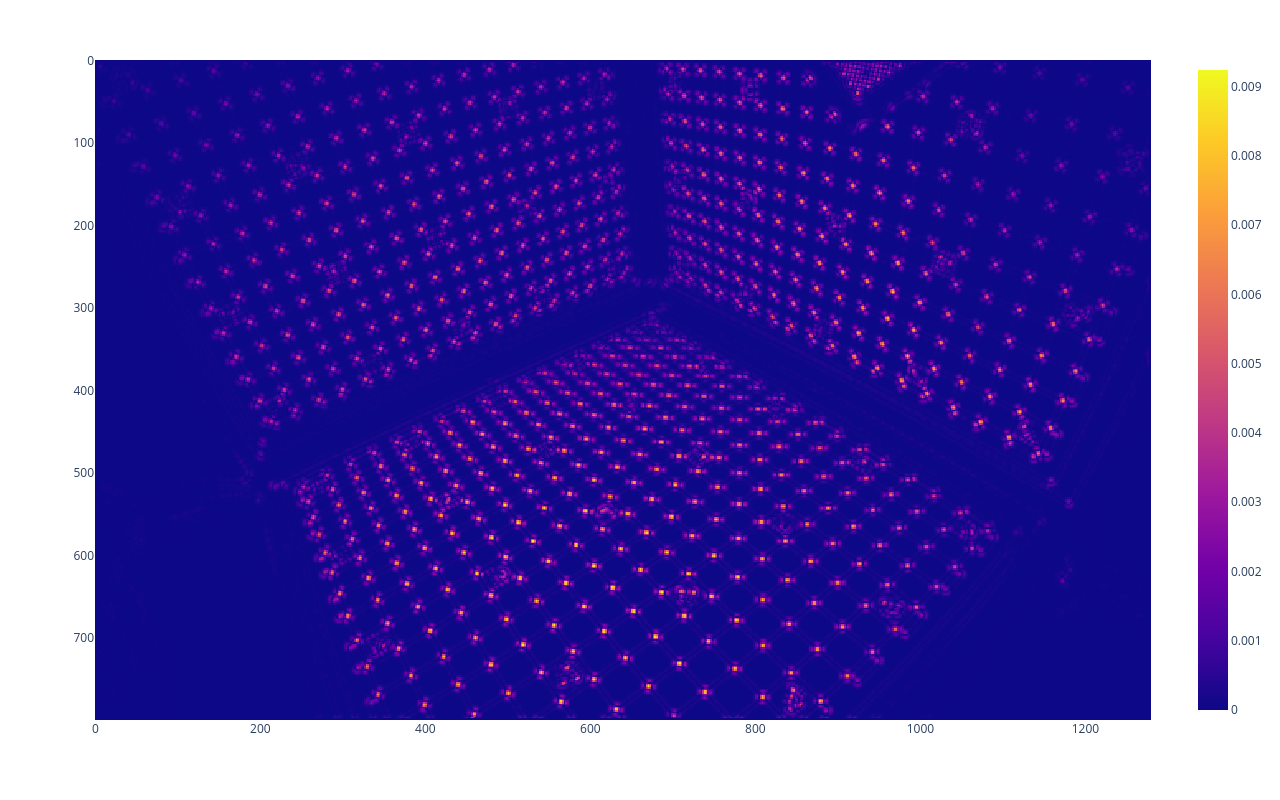
\includegraphics[width=\linewidth]{response_hessian.png}
	\captionof{figure}{Hessian response}
	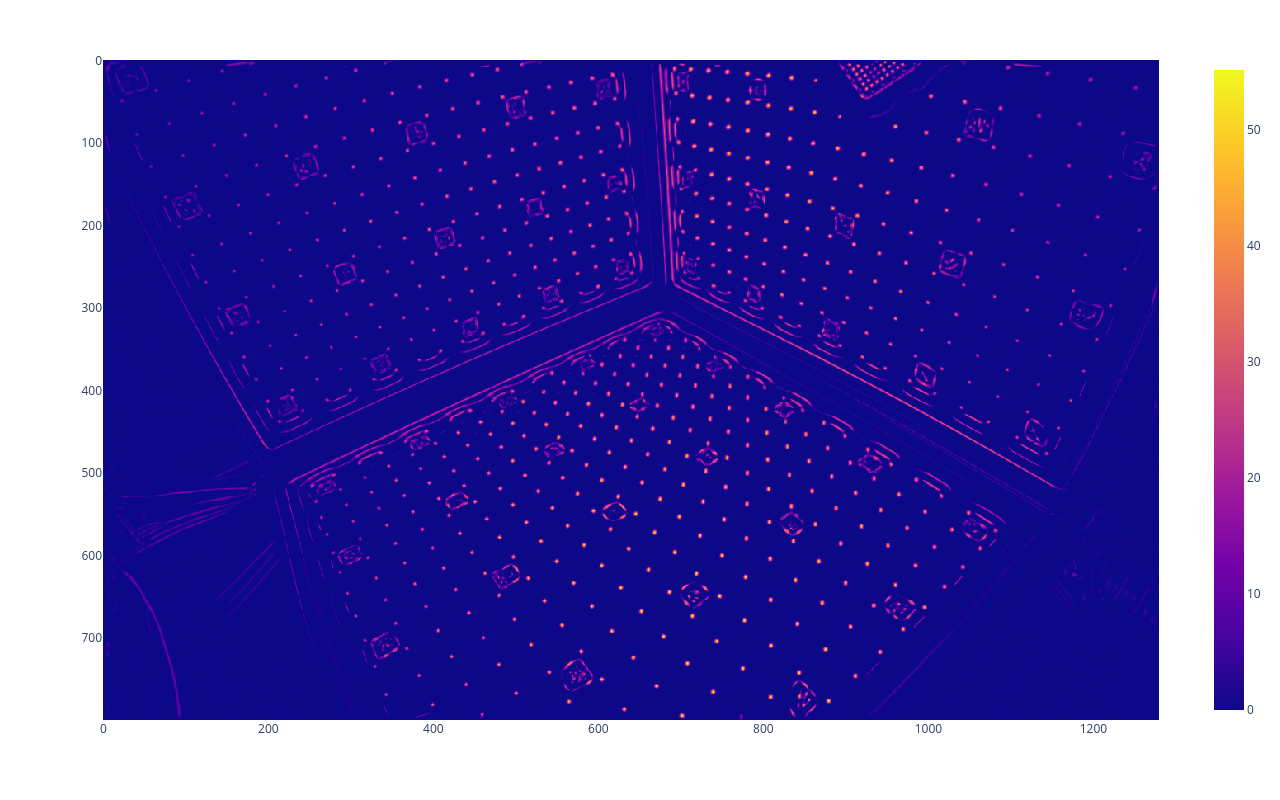
\includegraphics[width=\linewidth]{response_other.png}
	\captionof{figure}{Response used by \cite{geigerAutomaticCameraRange2012}}
	% \end{figure}
\end{minipage}

\begin{figure}
	\centering
	\begin{subfigure}[t]{\linewidth}
		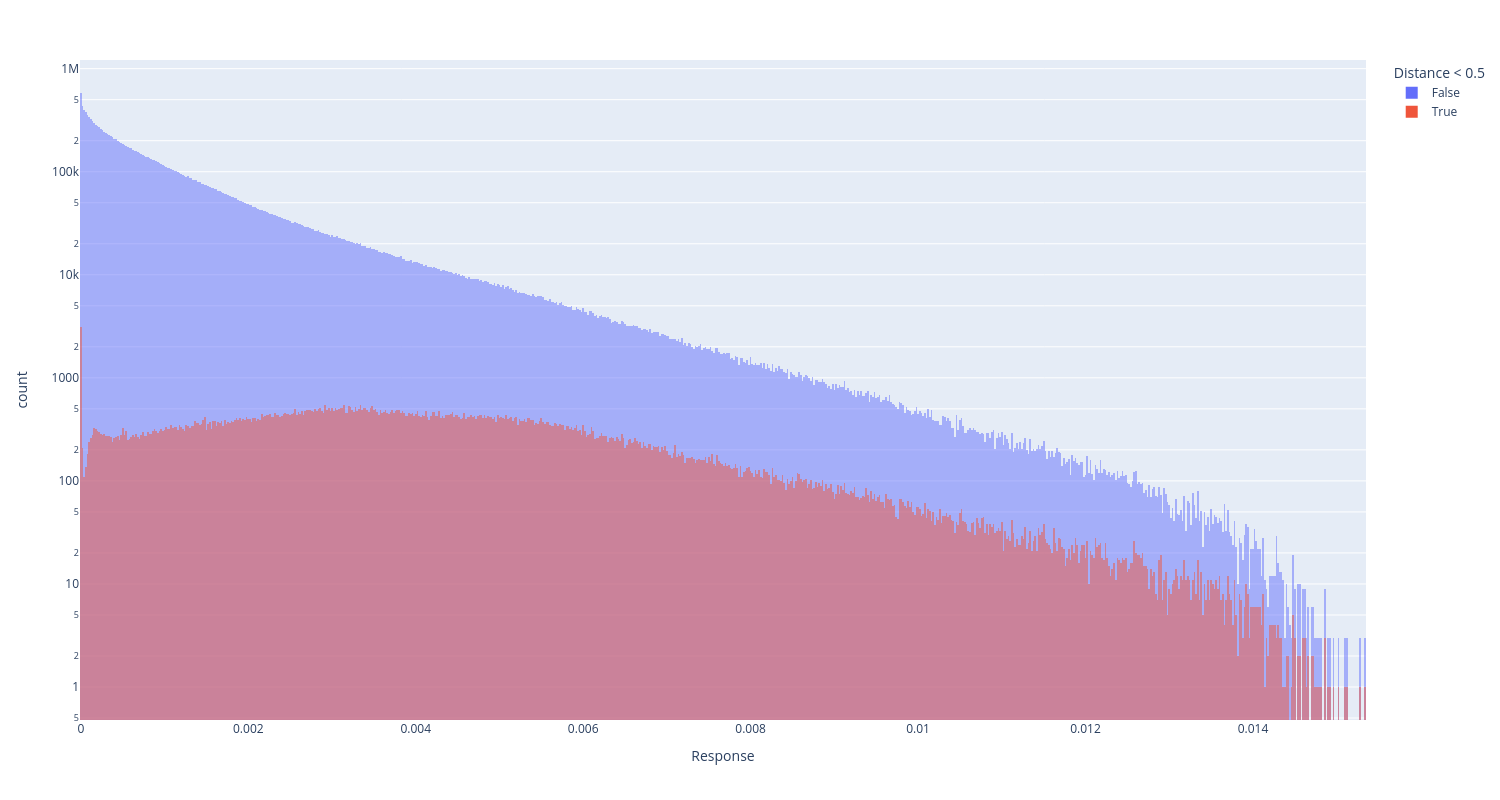
\includegraphics[width=\linewidth]{hist_response_hessian.png}
		\caption{Histogram of Hessian response}
	\end{subfigure}
	\begin{subfigure}[t]{\linewidth}
		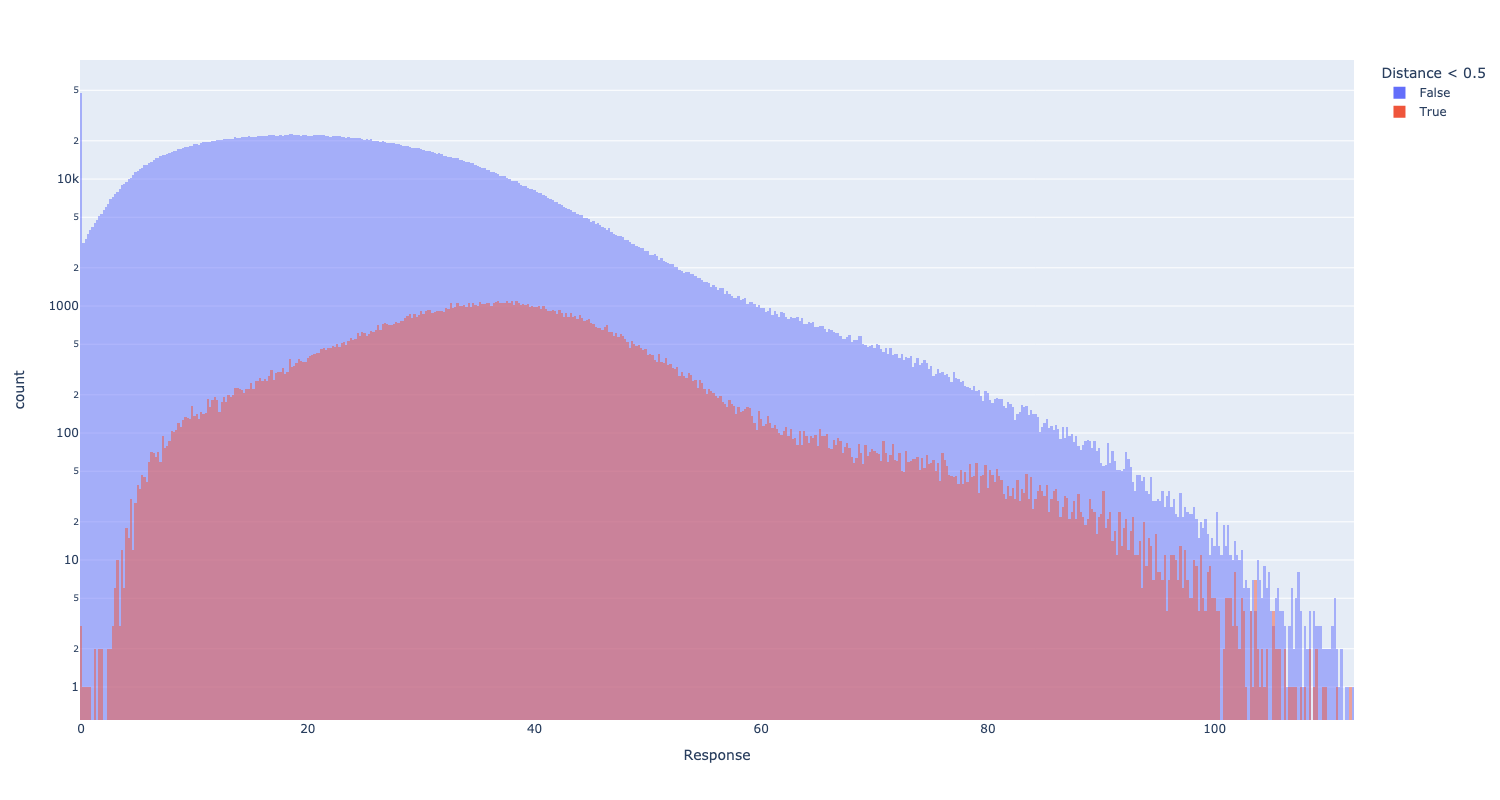
\includegraphics[width=\linewidth]{hist_response_other.png}
		\caption{Histogram of response used by \cite{geigerAutomaticCameraRange2012}}
	\end{subfigure}
	\caption{Distributions of the responses for the image on the
		\cref{fig:extended_board_img}. Note the log y-scale! Most of the points have
		the response 0.}
\end{figure}

\section{Evaluation}\label{sec:evaluation}

\subsection{Recovery of artificially removed points}\label{sub:recovery_of_artificially_removed_points}

We removed 20\% of the points from the original board, and then tried to recover
them.

\begin{figure}
  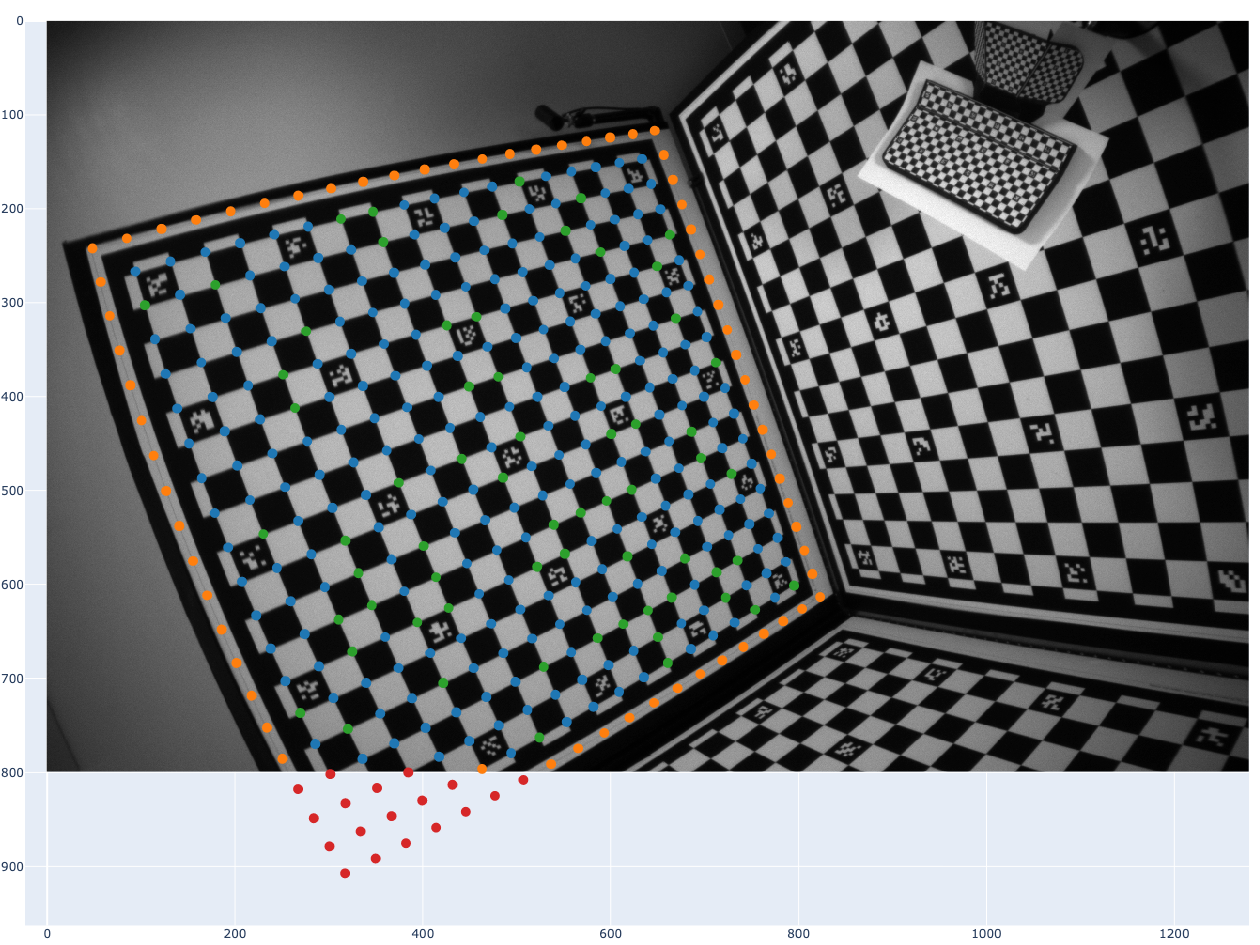
\includegraphics[width=\linewidth]{refined_pruned_corners.png}
  \caption{Recovered occluded points}
\end{figure}

\begin{figure}[h]
	\begin{tikzpicture}
		\begin{axis}[
				ybar interval,
				ymin=0,
				ylabel={Frequency},
				xlabel={Value},
				height=0.3\linewidth,
				width=\linewidth,
				ticklabel style = {font=\tiny},
				% title={Initial calibration}
			]
			\addplot+ [hist={data min=0,data max=500,bins=20}] table [y index=0]
				% \addplot+ [hist={bins=30}] table [y index=0]
				{data/pruned_number_of_features.txt};
		\end{axis}
	\end{tikzpicture}
	\caption{Initial calibration's reprojection error histogram}
\end{figure}
\begin{figure}[h]
	\begin{tikzpicture}
		\begin{axis}[
				ybar interval,
				ymin=0,
				ylabel={Frequency},
				xlabel={Value},
				height=0.3\linewidth,
				width=\linewidth,
				ticklabel style = {font=\tiny},
				% title={Reprojection error}
			]
			\addplot+ [hist={data min=0,data max=500,bins=20}] table [y index=0]
				% \addplot+ [hist={bins=30}] table [y index=0]
				{data/recovered_pruned_number_of_features.txt};
		\end{axis}
	\end{tikzpicture}
	\caption{Final calibration's reprojection error histogram}
\end{figure}

\subsection{Performance under occlusion}\label{sub:performance_under_occlusion}

Occlusions pose additional complications for the feature detection. We added an
image on top of the board, and tried to recover additional points. Often the
initial feature detector failed to detect points near the occlusion.

\begin{figure}
  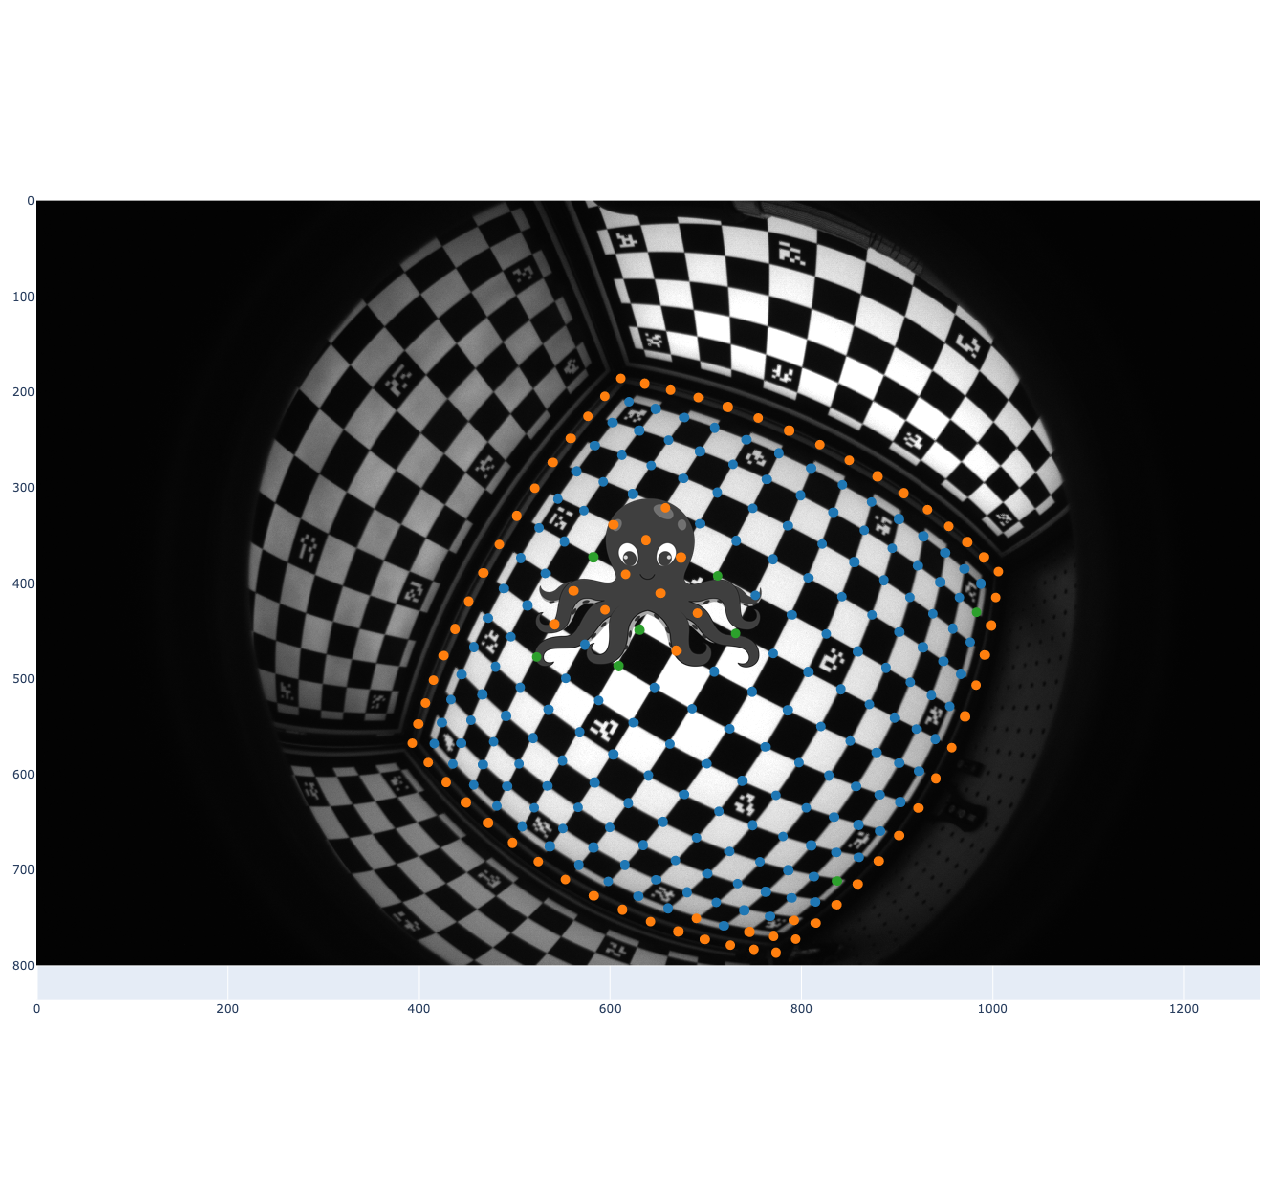
\includegraphics[width=\linewidth]{refined_overlayed_corners.png}
  \caption{Recovered occluded points}
\end{figure}

\begin{figure}[h]
	\begin{tikzpicture}
		\begin{axis}[
				ybar interval,
				ymin=0,
				ylabel={Frequency},
				xlabel={Value},
				height=0.3\linewidth,
				width=\linewidth,
				ticklabel style = {font=\tiny},
				% title={Initial calibration}
			]
			\addplot+ [hist={data min=0,data max=500,bins=20}] table [y index=0]
				% \addplot+ [hist={bins=30}] table [y index=0]
				{data/occluded_number_of_features.txt};
		\end{axis}
	\end{tikzpicture}
	\caption{Initial calibration's reprojection error histogram}
\end{figure}
\begin{figure}[h]
	\begin{tikzpicture}
		\begin{axis}[
				ybar interval,
				ymin=0,
				ylabel={Frequency},
				xlabel={Value},
				height=0.3\linewidth,
				width=\linewidth,
				ticklabel style = {font=\tiny},
				% title={Reprojection error}
			]
			\addplot+ [hist={data min=0,data max=500,bins=20}] table [y index=0]
				% \addplot+ [hist={bins=30}] table [y index=0]
				{data/recovered_occluded_number_of_features.txt};
		\end{axis}
	\end{tikzpicture}
	\caption{Final calibration's reprojection error histogram}
\end{figure}

\subsection{Recovery of previously undetected points}\label{sub:recovery_of_previously_undetected_points}

\missingfigure{Compare the number of points with the provided by babelcalib}
\missingfigure{Compare the reprojection error}


